\documentclass[a4paper,10pt]{article}
\usepackage[margin=1.8cm]{geometry}
\usepackage{graphicx}
\usepackage{tikz}
\usepackage{enumitem}
\usepackage{multicol}
\usepackage{booktabs}
\usepackage{hyperref}
\usepackage{xcolor}
\usepackage{titlesec}
\usepackage{parskip}
\usepackage{mdframed}
\usetikzlibrary{shapes.geometric, arrows.meta, positioning, decorations.pathreplacing}

\titlespacing{\section}{0pt}{6pt}{3pt}
\titlespacing{\subsection}{0pt}{4pt}{2pt}
\setlength{\parskip}{3pt}

\hypersetup{colorlinks=true, linkcolor=blue, urlcolor=blue}

\title{\vspace{-1.5cm}\textbf{Movie Rating Analysis and Visualization}\\
\large Milestone 2 --- COM-480 Data Visualization\\[2pt]
\normalsize Group: Sarah Le Duc \quad|\quad
Yassine Alaoui (358113), Amine Louah (343896), Sarah Lim (341929), Ilian Changkakoti (340815)}
\date{}

\begin{document}
\maketitle
\vspace{-0.8cm}
\hrule
\vspace{0.3cm}

%% ─────────────────────────────────────────────────────────
\section{Project Goal}

Our goal is an interactive website that lets users explore how movies are evaluated
across rating systems (IMDb user scores vs.\ Metacritic critic scores) and platforms
(IMDb Top 1000 vs.\ Netflix catalog). We focus on \emph{disagreements}: where
audiences and critics diverge, how genre popularity shifts over decades, and what
separates ``crowd favorites'' from ``critical darlings.''

Following MS1 feedback, we address dataset imbalance explicitly: the IMDb Top
1000 is a curated high-rating slice ($\mu \approx 7.95$), while Netflix is broad
and heterogeneous ($\mu \approx 6.53$). Comparisons are made within matched
subsets (movies present in both, same genre/decade strata) to avoid misleading
cross-dataset averages.

%% ─────────────────────────────────────────────────────────
\section{Visualization Sketches, Tools \& Lectures}

\begin{multicols}{2}

\subsection*{V1 — Dumbbell Plot: Audience vs.\ Critic}

\begin{center}
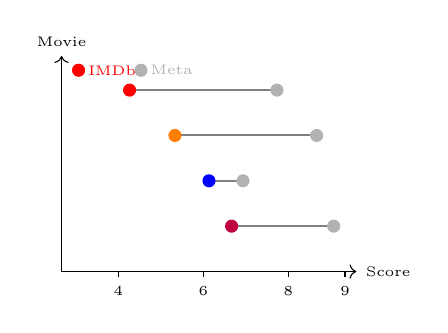
\begin{tikzpicture}[scale=0.72]
  % axes
  \draw[->] (0,0) -- (5.2,0) node[right,font=\tiny] {Score};
  \draw[->] (0,0) -- (0,3.8) node[above,font=\tiny] {Movie};
  % tick labels
  \foreach \x/\lbl in {1/4,2.5/6,4/8,5/9}
    \draw (\x,0) -- (\x,-0.1) node[below,font=\tiny] {\lbl};
  % dumbbell rows
  \foreach \y/\a/\b/\col in {
    3.2/1.2/3.8/red,
    2.4/2.0/4.5/orange,
    1.6/2.6/3.2/blue,
    0.8/3.0/4.8/purple}
  {
    \draw[gray,line width=0.7pt] (\a,\y) -- (\b,\y);
    \filldraw[\col] (\a,\y) circle (3pt);
    \filldraw[gray!60] (\b,\y) circle (3pt);
  }
  % legend
  \filldraw[red] (0.3,3.55) circle (3pt) node[right,font=\tiny] {IMDb};
  \filldraw[gray!60] (1.4,3.55) circle (3pt) node[right,font=\tiny] {Meta};
\end{tikzpicture}
\end{center}

Each movie is a horizontal segment connecting its IMDb user score (colored dot)
to its normalized Metacritic score (grey dot). Movies are sorted by gap magnitude,
making the most divisive titles immediately visible. A tooltip on hover reveals
title, genre, and year.

\textbf{Tools:} D3.js (force layout + transitions), HTML/CSS.\\
\textbf{Lectures:} D3 intro, Interaction \& Perception, Color.

\subsection*{V2 — Genre Bar-Chart Race}

\begin{center}
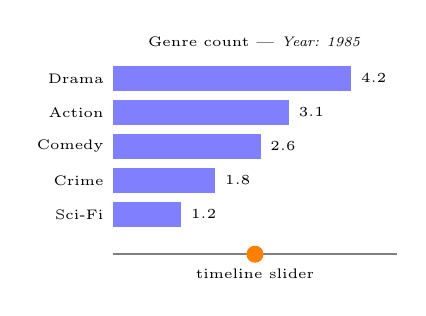
\begin{tikzpicture}[scale=0.72]
  % title
  \node[font=\tiny] at (2.5,3.65) {Genre count --- \textit{Year: 1985}};
  % bars
  \foreach \y/\w/\lbl in {
    3.0/4.2/Drama,
    2.4/3.1/Action,
    1.8/2.6/Comedy,
    1.2/1.8/Crime,
    0.6/1.2/Sci-Fi}
  {
    \fill[blue!50] (0,\y-0.22) rectangle (\w,\y+0.22);
    \node[left,font=\tiny] at (0,\y) {\lbl};
    \node[right,font=\tiny] at (\w,\y) {\pgfmathprintnumber{\w}};
  }
  % slider
  \draw[thick,gray] (0,-0.1) -- (5,-0.1);
  \filldraw[orange] (2.5,-0.1) circle (4pt);
  \node[font=\tiny] at (2.5,-0.45) {timeline slider};
\end{tikzpicture}
\end{center}

A horizontal bar chart that animates as a year slider moves from 1920 to 2023.
Bar lengths encode the count (or average rating) of each genre per decade.
A play/pause button drives the animation; clicking a bar filters V1 and V3.

\textbf{Tools:} D3.js (transitions, \texttt{d3-timer}), Svelte (state management).\\
\textbf{Lectures:} Animation \& Storytelling, Interaction.

\subsection*{V3 — Hexbin Density Map}

\begin{center}
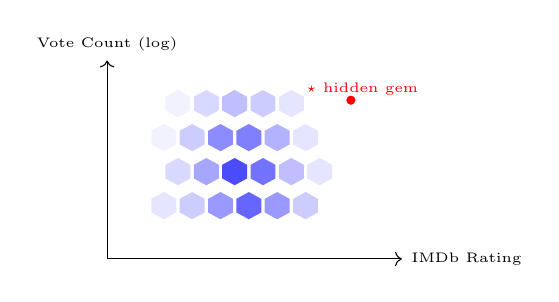
\begin{tikzpicture}[scale=0.72]
  \draw[->] (0,0) -- (5.2,0) node[right,font=\tiny] {IMDb Rating};
  \draw[->] (0,0) -- (0,3.5) node[above,font=\tiny] {Vote Count (log)};
  % hex grid mockup
  \foreach \cx/\cy/\col in {
    1.0/0.7/blue!10, 1.5/0.7/blue!20, 2.0/0.7/blue!40,
    2.5/0.7/blue!60, 3.0/0.7/blue!40, 3.5/0.7/blue!20,
    1.25/1.3/blue!15, 1.75/1.3/blue!35, 2.25/1.3/blue!70,
    2.75/1.3/blue!55, 3.25/1.3/blue!25, 3.75/1.3/blue!10,
    1.0/1.9/blue!5,  1.5/1.9/blue!20,  2.0/1.9/blue!45,
    2.5/1.9/blue!50, 3.0/1.9/blue!30,  3.5/1.9/blue!10,
    1.25/2.5/blue!5, 1.75/2.5/blue!15, 2.25/2.5/blue!25,
    2.75/2.5/blue!20, 3.25/2.5/blue!10}
  {
    \fill[\col] (\cx,\cy) -- ++(0.22,0.12) -- ++(0,0.24) -- ++(-0.22,0.12)
                          -- ++(-0.22,-0.12) -- ++(0,-0.24) -- cycle;
  }
  % outlier label
  \node[red,font=\tiny] at (4.5,3.0) {$\star$ hidden gem};
  \filldraw[red] (4.3,2.8) circle (2pt);
\end{tikzpicture}
\end{center}

A hexbin chart plotting \textbf{IMDb rating} (x-axis) vs.\ \textbf{log vote
count} (y-axis), colored by bin density. A decade selector updates the hexbins.
Outlier movies above the main cluster (high rating, low votes) are highlighted as
``hidden gems.'' A toggle switches between IMDb Top 1000 and Netflix subsets.

\textbf{Tools:} D3-hexbin plugin, D3.js.\\
\textbf{Lectures:} Perception \& Color, Marks \& Channels, Tabular Data.

\end{multicols}

%% ─────────────────────────────────────────────────────────
\section{Implementation Breakdown}

\begin{center}
\renewcommand{\arraystretch}{1.15}
\begin{tabular}{@{}p{0.24\linewidth}p{0.37\linewidth}p{0.30\linewidth}@{}}
\toprule
\textbf{Component} & \textbf{Core MVP (required)} & \textbf{Extra / Enhancement} \\
\midrule
\textbf{Data pipeline} &
  Merge IMDb + Netflix on title/year; normalize scores to $[0,10]$; flag
  matched vs.\ unmatched entries; export cleaned JSON for D3 &
  Enrich with TMDB API (posters, box office); add confidence bands based
  on vote-count reliability \\
\addlinespace
\textbf{V1 Dumbbell} &
  Static dumbbell sorted by gap; hover tooltip (title, year, genre, scores) &
  Animated entry on scroll; click-to-search IMDB; color by genre \\
\addlinespace
\textbf{V2 Bar Race} &
  Animated bar chart with play/pause slider across decades &
  Cross-link with V3 (selecting a genre highlights hexbins); speed control \\
\addlinespace
\textbf{V3 Hexbin} &
  Hexbin of rating vs.\ vote count for one dataset at a time &
  Side-by-side IMDb vs.\ Netflix panels; lasso selection exports a filtered
  movie list \\
\addlinespace
\textbf{Global filters} &
  Genre selector; year range slider &
  Full-text search; ``surprise me'' random highlight; share-URL state \\
\bottomrule
\end{tabular}
\end{center}

\vspace{0.2cm}

\noindent\textbf{Addressing dataset bias (MS1 feedback):} All cross-dataset
comparisons use only the \emph{intersection} of titles present in both datasets
($n \approx 400$--500 after matching). Genre/decade distributions are shown
separately per source alongside any combined view, and tooltips surface the
underlying $n$ for every aggregate so users can judge the reliability of each
visual encoding themselves.

%% ─────────────────────────────────────────────────────────
\section{Functional Prototype}

The website is live at \url{https://github.com/com-480-data-visualization/project-2025-sarah_le_duc}.
It currently contains:
\begin{itemize}[nosep,leftmargin=*]
  \item A landing \textbf{Overview} tab with project description, key research
        questions, and a summary statistics table comparing both datasets.
  \item \textbf{V1 — Dumbbell plot} fully functional: loads real IMDb data,
        supports genre filter, top-$N$ selector, and four sort modes; hover
        tooltip shows title, year, genre, both scores, and vote count.
  \item \textbf{V2 — Genre Bar-Chart Race} fully functional: animated horizontal
        bar chart driven by a decade slider (1920s--2020s) with Play/Pause; supports
        movie-count and average-IMDb-rating metrics; smooth D3 transitions reorder
        genres each decade.
  \item \textbf{V3 — Hexbin Density Map} fully functional: hexagonal bins coloured
        by movie density on the IMDb-rating $\times$ log-vote-count plane; decade
        and genre filters; ``hidden gem'' overlay highlights high-rated
        (\(\geq 8.0\)) but underexposed (\(<\)100k votes) titles in gold.
  \item Cleaned CSV data files (\texttt{imdb\_top1000\_cleaned.csv},
        \texttt{netflix\_cleaned.csv}) generated from the Jupyter preprocessing
        notebook; loaded at runtime via \texttt{d3.csv()}.
  \item D3.js v7 and the \texttt{d3-hexbin} plugin loaded via CDN; a shared
        tooltip and data-cache layer (\texttt{main.js}) serves all three views.
\end{itemize}

\end{document}
